\section{Supervised Learning}
\label{sec:supervised}
Searches for specific signatures or interactions in collider data can in general be thought of as a classification problem - some known signal process must be identified and separated from some known and well-modeled set of background processes. Any iterative algorithm can then improve its ability to properly identify signal from background by comparing its predictions to the true known classifications and adjusting its internal parameters. This type of approach is known as supervised machine learning, and it is particulary relevant for measuring dihiggs decays. 

% BDT
\subsection{Boosted Decision Trees}
\label{sec:BDT}
Boosted Decision Trees (BDTs) have a long history in high energy physics from enabling the first observation of single top production at the Tevatron~\cite{Abazov:2006gd, Aaltonen:2008sy} to helping in the discovery of the Higgs boson at the LHC~\cite{Aad_2012, Chatrchyan_2012}. A decision tree functions by making a series of cuts (or decisions) that maximize the separation between signal and background events in a single dimension. Each cut produces a branch in the tree containing independent populations. The depth of the tree sets the number of decisions a tree will make, and a well-designed tree will have end-nodes that efficiently separate and properly identify the constituent classes. Any series of cuts for identifying events will inevitably misclassify some events, and there are many strategies for improving the results. A boosted decision tree attempts to improve the classification by creating a new set of data from the improperly classified events and training a new decision tree on these inputs. Each step of re-training with misclassified events is called a \textit{boost}, and the total prediction for an event is the weighted sum of predictions from the orignal tree and the boosted trees where each sequential boost recieves a smaller weight in the sum.

The BDT trained for di-Higgs detection was built using the xgboost package~\cite{xgboost}. The top seventeen reconstructed and event-level variables ranked by KS separability (discussed in Section~\ref{sec:eventReco}) were used in training. The hyperparameters describing the boosted decision tree were optimized for maximum $S/\sqrt{B}$. The optimal hyperparamters were found to be as follows: multiplicative boost factor of 0.1, maximum tree depth of 9, gamma (minimum loss reduction needed for further partition) of 1.1, and an L2 regularization term of 8.28.

\begin{figure}[!h]
\begin{center}
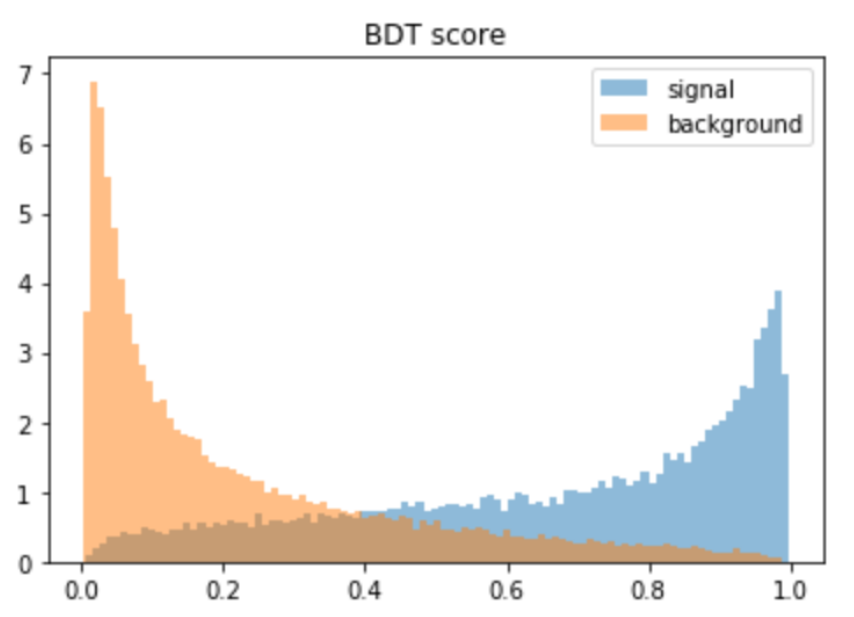
\includegraphics[width=3in]{BDT/bdt_pred}
\caption{Signal predictions of the trained BDT for signal and background samples independent from the training sets.}
\label{fig:bdt_pred}
\end{center}
\end{figure}

The predictions from the optimized BDT are shown in Figure~\ref{fig:bdt_pred}. A maximum significance of 1.84$\pm$0.09 was obtained, yielding 986 signal events and 2.8$\cdot 10^5$ background events. 


% ff Neural Network
\subsection{Feed Forward Neural Network}
\label{sec:NN}
Fully connected or feed-forward neural networks (NNs) also have a long history in high energy physics. The fundamental element of any neural network is called a \textit{layer}. Multiple layers are stacked together to produce a final prediction given the input variables from the first layer. This predicted outcome is then evaluated against a known target value. A fully-connected network can have multiple internal (or hidden) layers between the input and output layers, and each hidden layer is composed of a series of trainable activation functions and weights that allow the network to identify and iteratively combine important features of the input space. A function (called the loss function) is chosen to quantify the difference between the model prediction and target values. The loss calculated after a single training iteration is used to adjust the internal network weights in the next training iteration through a process called backpropagation. The model is fully trained once the improvement in the loss between iterations falls beneath some user-defined threshold.

The NN trained for di-Higgs detection was built using the Keras~\cite{chollet2015keras} and Tensorflow~\cite{tensorflow} packages. The top twenty-two most separable reconstructed and event-level variables were used as the input variables for the NN. The complete network structure consists of the input layer, two hidden layers, and a single-node output layer. The first hidden layer contains 175 nodes with an L2 kernel regularizer ($\lambda$ = $10^{-4}$). The second hidden layer contains 90 nodes with no kernel regularizer. A batch normalization layer and a dropout (0.2) function are placed in between the two hidden layers to prevent over-fitting. Both hidden layers use a rectified linear (ReLU) activation function, while the output layer uses a sigmoid activation function. Several models were trained by individually tuning each hyperparameter over a reasonable range in order to produce a final optimized model. A schematic flowchart of the network structure is shown in Figure~\ref{fig:nn}.
%The sequential model was compiled using the ‘adam’ optimizer along with the ‘binary\_crossentropy’ loss method. Finally, the model was fit on the training data along with the validation data for 100 epochs. 

\begin{figure}[!h] 
\begin{center}
\includegraphics*[width=0.75\textwidth] {ffNN/figures/flowchart_ffNN.png}
\caption{Structure of the feed-forward neural network. The input variables are fed through two fully connected dense layers to classify events. One dropout layer and one batch normalization layer help mitigate over-fitting during training.}
  \label{fig:nn}
\end{center}
\end{figure}

The NN was trained for 25 epochs before the minimal loss-improvement threshold was met, and the results are shown in Figure~\ref{fig:results_nn}. The trained model obtained a maximum $\sigma$ = 2.40$\pm$0.08 when considering events with a signal prediction score > 0.94. This phase-space has a signal yield of $1659.9 \pm 12.5$ events and a background yield of $4.8 \pm 0.2$ $\cdot$ $10^5$ events. %477215.3 events.

\begin{figure}[!h] 
\begin{center}
   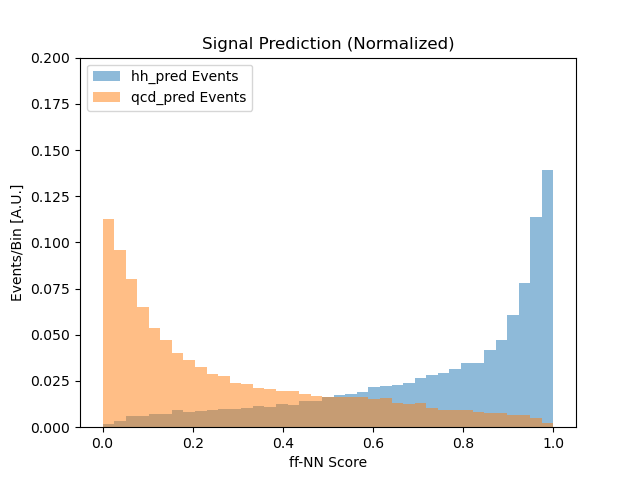
\includegraphics[width = 3in]{ffNN/figures/score_ffnn_v3}\\
\caption{Final predictions of the feed-forward network for signal and background samples.}
  \label{fig:results_nn}
\end{center}
\end{figure}



% ff Neural Network
\subsection{Convolutional Network}
\label{sec:CNN}
Convolutional Neural Networks (CNNs) are neural networks that predict the content of an input image by using assumptions about the local relationships between neighboring pixels. For this analysis, content prediction is simplified to a general classification of whether the image comes from a di-Higgs or QCD event. The fundamental elements of any convolutional network are convolutional layers and pooling layers. Convolutional layers use filters that perform linear combinations of neighboring pixels within the filter size, and pooling layers aggregate information by grouping neighboring pixels using either their maximum or average values. After some number of these layers, the output is flattened into a one-dimensional vector, and this flattened vector is pushed through a set of feed-forward layers in order to make a final output prediction. 

Many previous papers have explored the use of convolutional networks trained on low-level quantities (e.g. tracks and calorimeter deposits) for the purposes of object identification~\cite{Alison:2019kud} at colliders. This paper extends the application to event-level identification. Using low-level quantities removes the need to reconstruct higher-level objects like jets or jet pairs; only the detector-level measurements are required for image creation. The performance of four convolutional networks were studied in the context of di-Higgs identification. The first network used a 3-layer image composed of energy/momentum weighted tracks, electromagnetic calorimeter deposits, and hadronic calorimeter deposits. The second network uses the same three layers but appends additional global event-level information to the flattened vector after image processing and before the fully connected layers. Figures~\ref{fig:cnn_nominal} and \ref{fig:cnn_hybrid} depict both network structures. The third and fourth networks follow the same pattern as the previous two but with the addition of two image layers corresponding to longitudinal and transverse impact parameter-weighted track information.

\begin{figure}[!h] 
\begin{center}
\includegraphics*[width=0.75\textwidth] {CNN/figures/nominalCNN.png}
\caption{Structure of the nominal convolutional neural network. The input images are fed through two convolutional layers and a single max-pooling layer before being flattened into a one-dimensional vector. The flattened vector is then fed through one fully connected layer, a batch normalization layer, and a final fully connected layer before a final prediction is made.}
  \label{fig:cnn_nominal}
\end{center}
\end{figure}

\begin{figure}[!h] 
\begin{center}
\includegraphics*[width=0.75\textwidth] {CNN/figures/hybridCNN.png}
\caption{Structure of the hybrid convolutional neural network. The input images are fed through two convolutional layers and a single max-pooling layer before being flattened into a one-dimensional vector. Scaled user-specified variables (e.g. $H_{T}$) are then concatenated with the flattened image vector. The concatenated vector is then fed through one fully connected layer, a batch normalization layer, and a final fully connected layer before a final prediction is made.}
  \label{fig:cnn_hybrid}
\end{center}
\end{figure}

In order to produce coherent images, the center of mass and the center of momentum for each event are calculated. All constituents are then boosted longitudinally into the center of mass of the event and rotated in phi to the center of momentum. After this pre-processing, each image layer corresponds to a 31x31 pixel grid centered on the total activity in the event. Figure~\ref{fig:cnn_avgQCD} shows an average QCD image and Figure~\ref{fig:cnn_avgDihiggs} shows an average di-Higgs image. While the average image layers for each sample closely resemble one another, they do contain different information, and variations are visible.

Importantly, clear differences are observed between the average QCD images and the average di-Higgs images. Each half of the di-Higgs image (split across $\phi$ = 0) is arranged in a roughly circular, isotropic shape due to the spin-0 nature of the Higgs. The QCD images appear balanced because of the effect of the pre-processing, but no similar circular structure is produced. Additionally, the variance of pixel intensities in di-Higgs images is much smaller than the variance in QCD images due to the more balanced kinematics of Higgs pair production compared to QCD processes.

\begin{figure}[!h] 
\begin{center}
  \subfloat[]{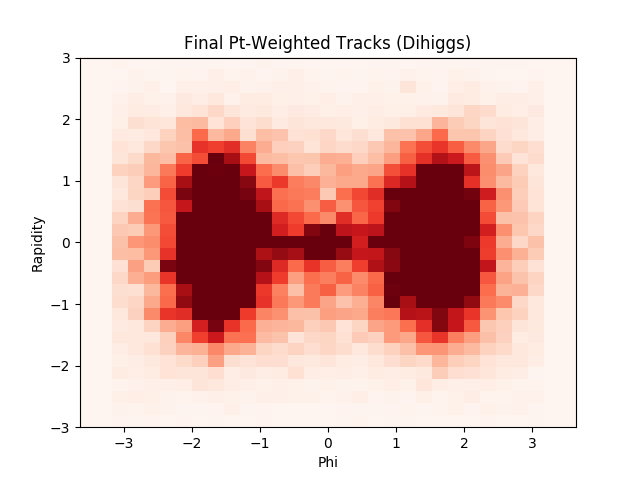
\includegraphics[width = 2in]{CNN/figures/images/qcd/Tracks_Dihiggs_Final_Pt-Weighted}} 
  \subfloat[]{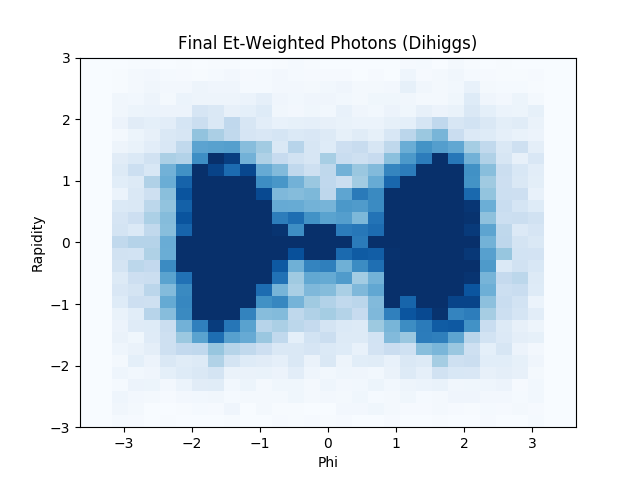
\includegraphics[width = 2in]{CNN/figures/images/qcd/Photons_Dihiggs_Final_Et-Weighted}}
  \subfloat[]{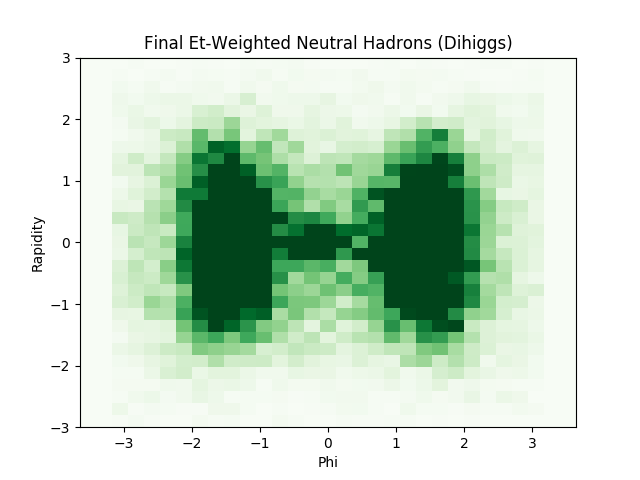
\includegraphics[width = 2in]{CNN/figures/images/qcd/NeutralHadrons_Dihiggs_Final_Et-Weighted}} \\
  \subfloat[]{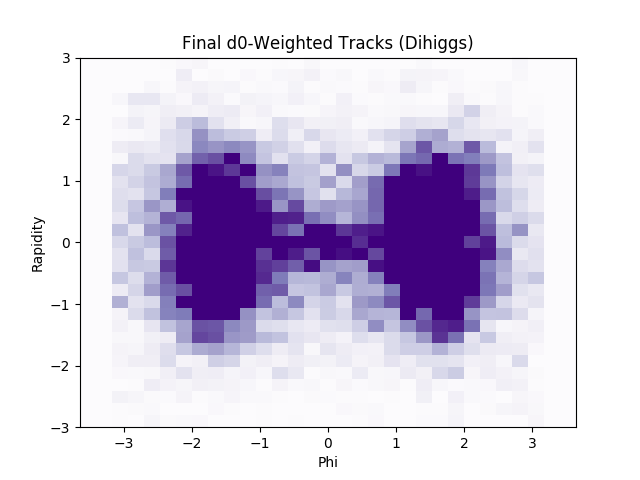
\includegraphics[width = 2in]{CNN/figures/images/qcd/Tracks_Dihiggs_Final_d0-Weighted}} 
  \subfloat[]{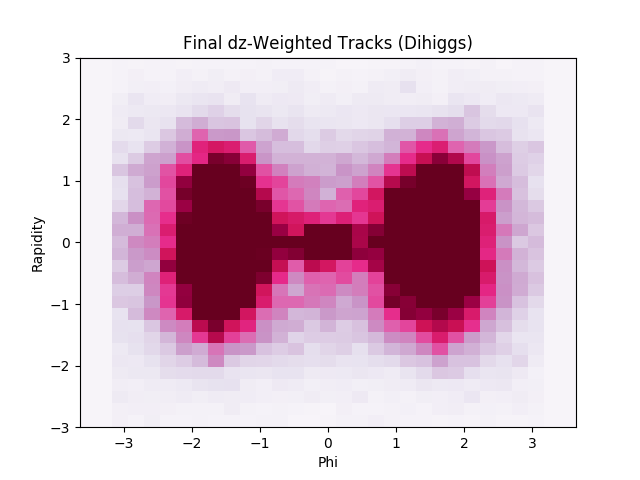
\includegraphics[width = 2in]{CNN/figures/images/qcd/Tracks_Dihiggs_Final_dz-Weighted}} 
\caption{Average QCD image showing (a) $p_{\textrm{T}}$-weighted tracks, (b) $E_{\textrm{T}}$-weighted ECAL deposits, (c) $E_{\textrm{T}}$-weighted HCAL deposits, (d) transverse impact parameter-weighted tracks, (e) longitudinal impact parameter-weighted tracks.}
\end{center}
\label{fig:cnn_avgQCD}
\end{figure}

\begin{figure}[!h] 
\begin{center}
  \subfloat[]{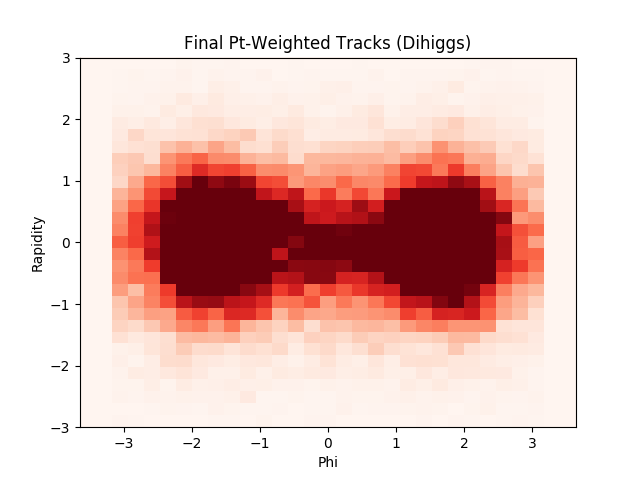
\includegraphics[width = 2in]{CNN/figures/images/hh/Tracks_Dihiggs_Final_Pt-Weighted}} 
  \subfloat[]{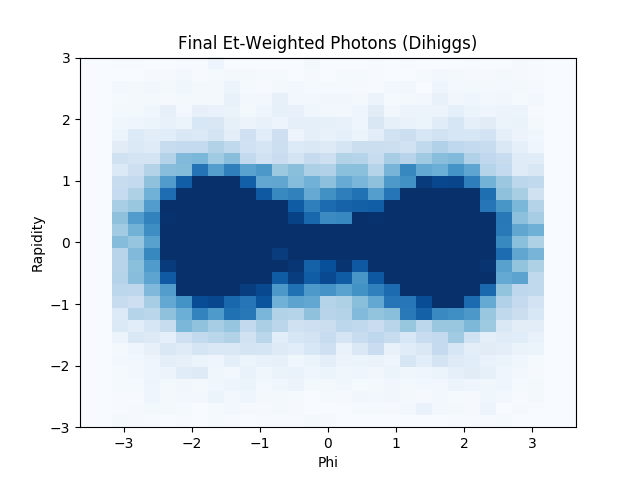
\includegraphics[width = 2in]{CNN/figures/images/hh/Photons_Dihiggs_Final_Et-Weighted}}
  \subfloat[]{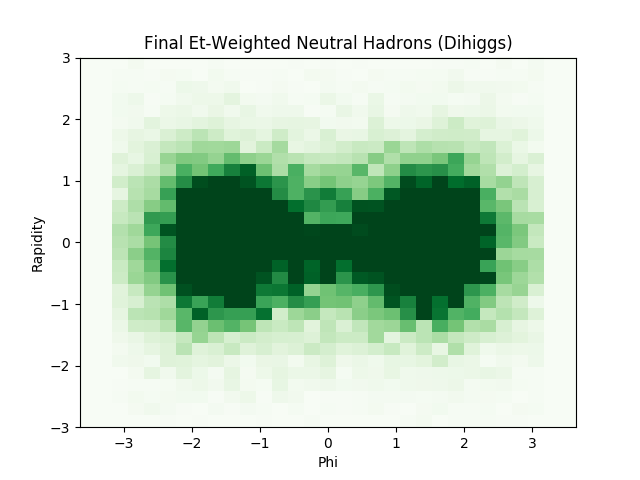
\includegraphics[width = 2in]{CNN/figures/images/hh/NeutralHadrons_Dihiggs_Final_Et-Weighted}} \\
  \subfloat[]{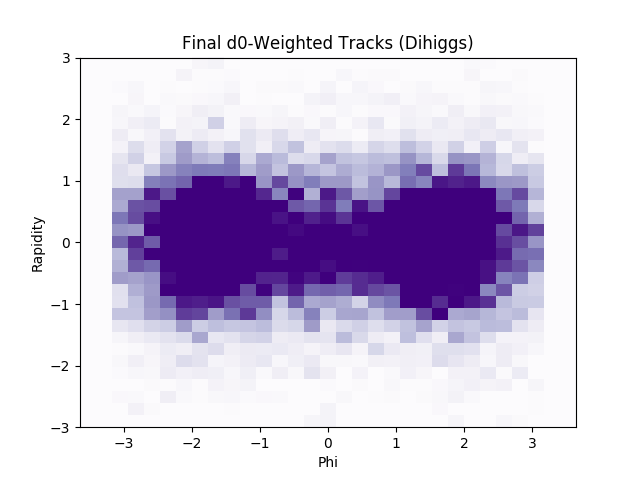
\includegraphics[width = 2in]{CNN/figures/images/hh/Tracks_Dihiggs_Final_d0-Weighted}} 
  \subfloat[]{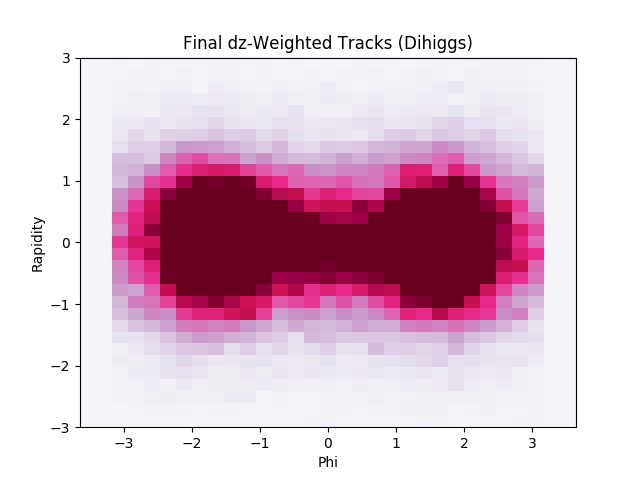
\includegraphics[width = 2in]{CNN/figures/images/hh/Tracks_Dihiggs_Final_dz-Weighted}} 
\caption{Average di-Higgs image showing (a) $p_{\textrm{T}}$-weighted tracks, (b) $E_{\textrm{T}}$-weighted ECAL deposits, (c) $E_{\textrm{T}}$-weighted HCAL deposits, (d) transverse impact parameter-weighted tracks, (e) longitudinal impact parameter-weighted tracks.}
\end{center}
\label{fig:cnn_avgDihiggs}
\end{figure}

As shown in Figures~\ref{fig:cnn_nominal} and \ref{fig:cnn_hybrid}, the CNN network structure uses two sequential 2D convolutional layers each with 16 3x3 filters, one max-pooling layer with a 2x2 window, a flattening of the outputs, two 64-node fully connected hidden layers, and one output layer for making the final prediction. As previously described, two of the networks append additional high level variables (scalar sum of transverse hadronic energy, number of jets, and number of $b$-tags) after the flattening and before the image information is fed through the fully connected layers. The optimal significance for each network is shown in Table~\ref{tab:cnnResults}. The best results were obtained using the 5-color network with additional high-level inputs, and the final predictions for this configuration are shown in Figure~\ref{fig:cnn_preds}. A best significance of 2.86$\pm$0.03 was found for a prediction cut $>$ 0.94 with a signal yield of 1.0$\cdot 10^4$ events and a background yield of 1.3$\cdot 10^7$ events.

\begin{table}[h!]
\label{tab:cnnResults}
  \begin{center}
    \begin{tabular}{|l|c|c|} % <-- Alignments: 1st column left, 2nd middle and 3rd right, with vertical lines in between
      \hline\hline
      \textbf{Method} & Best $S/\sqrt{B}$ & AUC \\
      \hline
      Tracks+HCAL+ECAL & 1.77 $\pm$ 0.01 & 0.818 \\
      Tracks+HCAL+ECAL + high-level & 2.12 $\pm$ 0.01 & 0.846 \\
      Tracks+HCAL+ECAL+D0+DZ & 2.45 $\pm$ 0.02 & 0.863 \\
      Tracks+HCAL+ECAL+D0+DZ + high-level & 2.86 $\pm$ 0.03 & 0.882 \\

      \hline\hline
    \end{tabular}
    \caption{Normalized to full HL-LHC dataset of 3000 fb$^{-1}$}
  \end{center}
\end{table}


\begin{figure}[!h] 
\begin{center}
  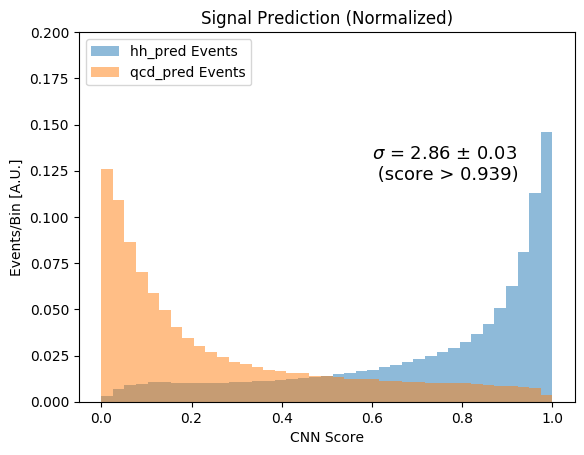
\includegraphics[width = 3in]{CNN/figures/5color_0PU_pix31_addHT-nJets-nBTags_2Conv16-16_one2DPool_EqualSamples/signal_CNNScore_norm}
  %\subfloat[]{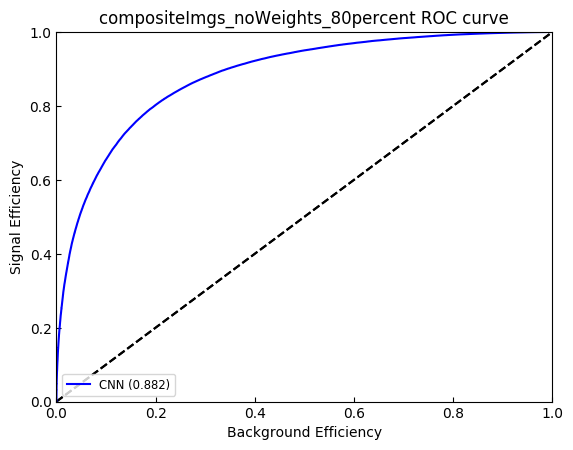
\includegraphics[width = 3in]{CNN/figures/5color_0PU_pix31_addHT-nJets-nBTags_2Conv16-16_one2DPool_EqualSamples/compositeImgs_noWeights_80percent_ROC}}\\
\caption{Signal prediction for the 5-color convolutional network with additional high-level inputs. The total area of the signal and background predictions are normalized to unity for easier shape comparison.}
\end{center}
\label{fig:cnn_preds}
\end{figure}



%\subsection{Residual Network}

\subsection{Lorentz Boost Network}
\label{sec:LBN}
a lorentz boost network? sounds cool, what's that?


% EFN network
\subsection{Energy Flow Network}
\label{sec:EFN}
Energy Flow Networks (EFN) and Particle Flow Networks (PFN) are algorithms that take basic jet constituents information as input rather than reconstructed jets and multi-jet composites, e.g. Higgs candidates. The EFN structure takes only the rapidity ${y}$ and azimuthal angle ${\phi}$ of jet constituents as input, while the PFN takes the rapidity $y$, azimuthal angle $\phi$, and transverse momentum $p_{T}$ of jet constituents as input. Using the constituents as input means no high level reconstruction is necessary when identifying events. Both the EFN and PFN are two-component networks, and their internal structures are shown in Figure \ref{fig:EFNArch}. The implementations of the EFN and PFN used for di-Higgs classification use 200 nodes for each hidden layer in network (a), 256 for latent space dimension and 300 nodes for each hidden layer in network (b). 

\begin{figure}[ht!]
\centering
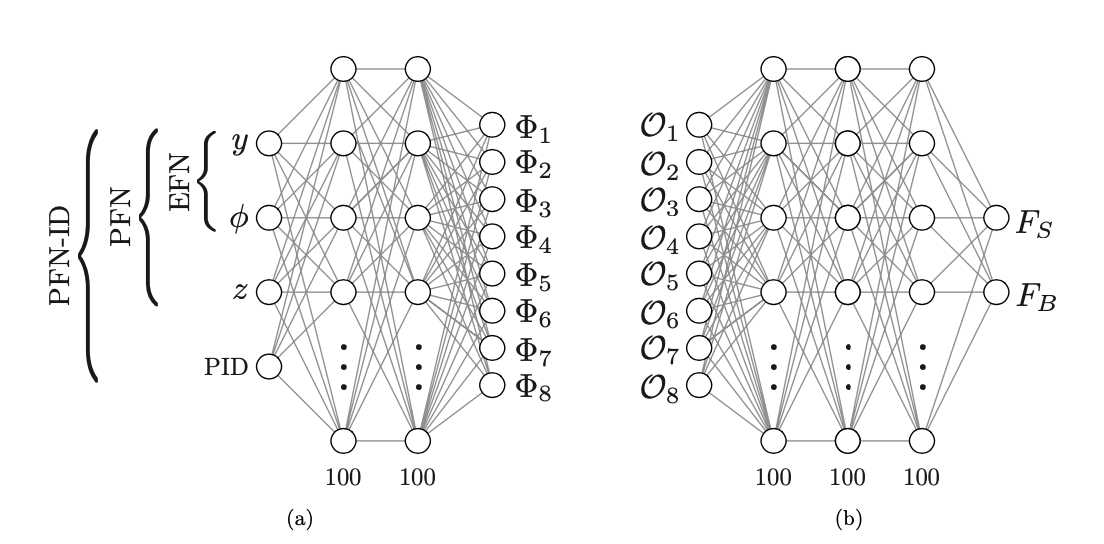
\includegraphics[scale=0.5]{./EFN/EFNArch.png}
\caption{Network (a) takes jet constituents information as input and outputs latent space $\Phi$ for each jet constituents. Network (b) takes $\mathcal{O}$, which is the linear combination of $\Phi$, as input and outputs final result.}
\label{fig:EFNArch}
\end{figure}

The EFN/PFN networks were trained using four separate categories split by number of jets and number of $b$-tags in order to test the network's dependence on higher-level jet information. Independent networks were trained using: all events, only events with $\geq$4 jets, only events with $\geq$4 jets and =2 $b$-tags, and only events with $\geq$4 jets and $\geq$4 $b$-tags. In each configuration, the number of signal and background events were adjusted to maintain an equal proportion of each population in the training sample. L2 regularization and dropout layers were added to minimize over-fitting. The results obtained with the EFN are shown in Table~\ref{EFNtab}. The results of the PFN are shown in Table~\ref{PFNtab}.

\begin{table}[ht!]
\centering
  %\begin{center}
    \begin{tabular}{|l|c|c|c|} % <-- Alignments: 1st column left, 2nd middle and 3rd right, with vertical lines in between
      \hline\hline
      \multirow{2}{*}{\textbf{Category}} & \multicolumn{3}{c|}{0PU}\\
      \cline{2-4}
      & Best $S/\sqrt{B}$ & \textbf{N$_{\mathrm{Signal}}$} & \textbf{N$_{\mathrm{Background}}$} \\
      \hline
      All Events & $1.407 \pm 0.006$ & $1.89\cdot 10^4$ & $1.80\cdot 10^8$ \\
      4Jets & $1.363 \pm 0.006$ & $1.63\cdot 10^4$ & $1.43\cdot 10^8$ \\
      4Jets 2BTags & $1.343 \pm 0.006$ & $1.33\cdot 10^4$ & $9.95\cdot 10^7$ \\
      4Jets 4BTags & $0.867 \pm 0.008$ & $3468.65$ & $1.60\cdot 10^7$ \\
      \hline\hline
    \end{tabular}
    \caption{EFN results. Normalized to full HL-LHC dataset of 3000 fb$^{-1}$}
  %\end{center}
\label{EFNtab}
\end{table}

\begin{table}[ht!]
\centering
  %\begin{center}
    \begin{tabular}{|l|c|c|c|} % <-- Alignments: 1st column left, 2nd middle and 3rd right, with vertical lines in between
      \hline\hline
      \multirow{2}{*}{\textbf{Category}} & \multicolumn{3}{c|}{0PU}\\
      \cline{2-4}
      & Best $S/\sqrt{B}$ & \textbf{N$_{\mathrm{Signal}}$} & \textbf{N$_{\mathrm{Background}}$} \\
      \hline
      All Events & $1.618 \pm 0.008$ & $1.79\cdot 10^4$ & $1.21\cdot 10^8$ \\
      4Jets & $1.580 \pm 0.008$ & $1.32\cdot 10^4$ & $7.00\cdot 10^7$ \\
      4Jets 2BTags & $1.574 \pm 0.009$ & $1.32\cdot 10^4$ & $4.85\cdot 10^7$ \\
      4Jets 4BTags & $0.903 \pm 0.009$ & $3297.34$ & $1.33\cdot 10^7$ \\
      \hline\hline
    \end{tabular}
    \caption{PFN results. Normalized to full HL-LHC dataset of 3000 fb$^{-1}$}
  %\end{center}
\label{PFNtab}
\end{table}

Both networks performed best when trained over all events without any cuts on the number of jets or $b$-tags. The EFN obtained a highest significance of 1.41$\pm$0.01, and the PFN obtained a highest significance of 1.62$\pm$0.01.

